\documentclass{standalone}
\usepackage{standalone}

\begin{document}
\subsection{Mapper and Aligner}
The terms mapper and aligner often used alternatively\cite{mappingAndAlignment} to indicate a tool which align several portions of a read with several portions of a reference genome for certain reasons\cite{alignment}. But in recent days, these words carry a slightly different meaning. 

Mapper seeks for most matched clusters in the reference genome where the read could be fitted best. Based on some parameter it just identify most similar clusters which would help the aligner to align faster and easier. Figure \ref{fig:mapper} illustrates the concept.

On the other hand, aligner takes those mapping and align the read with the best suitable portion considering some insertion, deletion, mismatch if needed. Figure \ref{fig:aligner} shows a small demonstration where aligner picks one of the possible alignment and tells the read best fitted here, then stores this result in a specific format\cite{SAMformat}.

\begin{figure}
	\centering

	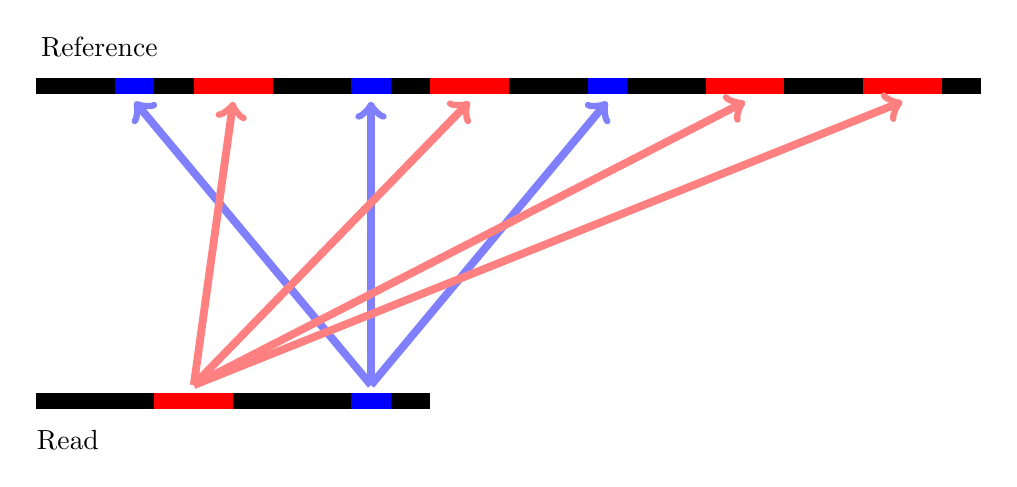
\begin{tikzpicture}[]
	
	%reference
	\draw[line width=2mm] (0,4) -- (12,4);
	\draw[line width=2mm,color=red] (2,4) -- (3,4);
	\draw[line width=2mm,color=red] (10.5,4) -- (11.5,4);
	\draw[line width=2mm,color=red] (8.5,4) -- (9.5,4);
	\draw[line width=2mm,color=red] (5,4) -- (6,4);
	\draw[line width=2mm,color=blue] (7,4) -- (7.5,4);
	\draw[line width=2mm,color=blue] (1,4) -- (1.5,4);
	\draw[line width=2mm,color=blue] (4,4) -- (4.5,4);
	%read
	\draw[line width=2mm] (0,0) -- (5,0);
	\draw[line width=2mm,color=red] (1.5,0) -- (2.5,0);
	\draw[line width=2mm,color=blue] (4,0) -- (4.5,0);
	%labels
	\node[rectangle](refer) at (0.8,4.5) {Reference};

	\node[rectangle](refer) at (0.4,-0.5) {Read};
	%arrows
	\draw[line width=1mm,color=blue!50,->] (4.25,0.2) -- (1.25,3.8);
	\draw[line width=1mm,color=blue!50,->] (4.25,0.2) -- (7.25,3.8);
	\draw[line width=1mm,color=blue!50,->] (4.25,0.2) -- (4.25,3.8);
	\draw[line width=1mm,color=red!50,->] (2,0.2) -- (2.5,3.8);
	\draw[line width=1mm,color=red!50,->] (2,0.2) -- (11,3.8);
	\draw[line width=1mm,color=red!50,->] (2,0.2) -- (9,3.8);
	\draw[line width=1mm,color=red!50,->] (2,0.2) -- (5.5,3.8);
	\end{tikzpicture}
	\caption{Mapping is just indicating the clusters of a large segment of the read in reference. The red large segment is found in four places in the reference where blue large segment is found in three places.} \label{fig:mapper}
\end{figure}
\begin{figure}
	\centering
	
	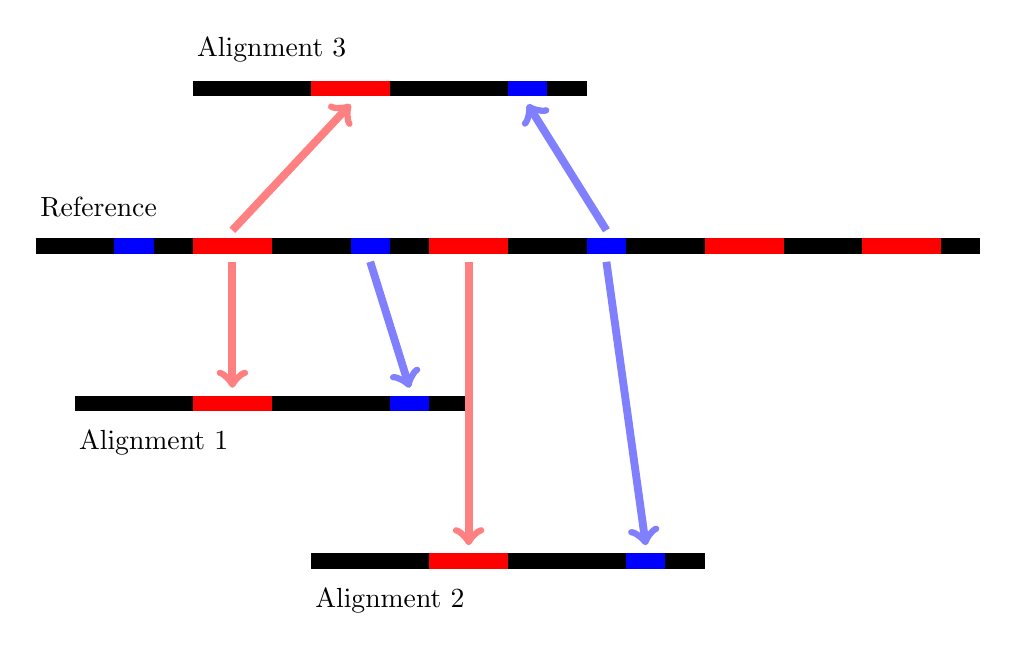
\begin{tikzpicture}[]
	
	%reference
	\draw[line width=2mm] (0,4) -- (12,4);
	\draw[line width=2mm,color=red] (2,4) -- (3,4);
	\draw[line width=2mm,color=red] (10.5,4) -- (11.5,4);
	\draw[line width=2mm,color=red] (8.5,4) -- (9.5,4);
	\draw[line width=2mm,color=red] (5,4) -- (6,4);
	\draw[line width=2mm,color=blue] (7,4) -- (7.5,4);
	\draw[line width=2mm,color=blue] (1,4) -- (1.5,4);
	\draw[line width=2mm,color=blue] (4,4) -- (4.5,4);
	%read 1
	\draw[line width=2mm] (0.5,2) -- (5.5,2);
	\draw[line width=2mm,color=red] (2,2) -- (3,2);
	\draw[line width=2mm,color=blue] (4.5,2) -- (5,2);
	%read 2
	\draw[line width=2mm] (3.5,0) -- (8.5,0);
	\draw[line width=2mm,color=red] (5,0) -- (6,0);
	\draw[line width=2mm,color=blue] (7.5,0) -- (8,0);
	%read 3
	\draw[line width=2mm] (2,6) -- (7,6);
	\draw[line width=2mm,color=red] (3.5,6) -- (4.5,6);
	\draw[line width=2mm,color=blue] (6,6) -- (6.5,6);
	%labels
	\node[rectangle](refer) at (0.8,4.5) {Reference};
	\node[rectangle](refer) at (1.5,1.5) {Alignment 1};
	\node[rectangle](refer) at (4.5,-0.5) {Alignment 2};
	\node[rectangle](refer) at (3,6.5) {Alignment 3};
	%arrows
	\draw[line width=1mm,color=red!50,->] (5.5,3.8) -- (5.5,0.2);
	\draw[line width=1mm,color=blue!50,->] (7.25,3.8) -- (7.75,0.2);
	\draw[line width=1mm,color=red!50,->] (2.5,3.8) -- (2.5,2.2);
	\draw[line width=1mm,color=blue!50,->] (4.25,3.8) -- (4.75,2.2);
	\draw[line width=1mm,color=red!50,->] (2.5,4.2) -- (4,5.8);
	\draw[line width=1mm,color=blue!50,->] (7.25,4.2) -- (6.25,5.8);
	\end{tikzpicture}
	\caption{Three possible alignment are showed based on the read mapping. The aligner does this type of alignment and picks most probable alignment based on several parameters.} \label{fig:aligner}
\end{figure}
\end{document}